General equation of circle is 
\begin{align}
    \vec{x}^T\vec{x}+ 2\vec{u}^T\vec{x}+f = 0
    \label{eq:solutions/1/6/eq:1}
\end{align}
The centre and the radius can be obtained as,
 \begin{align}
\vec{u}=\myvec{-1\\0}\\
f=-3\\
\vec{c}=-\vec{u}=\myvec{1\\0}\\
 r=\sqrt{\norm{\vec{u}}^2-f}=2
 \end{align}
$\because$ The tangents are parallel to the x-axis, their direction and normal vectors, $\vec{m}$ and $\vec{n}$ are respectively,
\begin{align}
\vec{m}=\myvec{1\\0}\\
\vec{n}=\myvec{0\\1}
\end{align}
For a circle, given the normal vector $\vec{n}$, the tangent points of contact to circle given by equation \eqref{eq:solutions/1/6/eq:1}  are given by
\begin{align}
    \vec{q_i}=(\kappa_i \vec{n}-\vec{u}), i=1,2
    \label{eq:solutions/1/6/eq:2}
\end{align}
where
\begin{align}
    \kappa_i=\pm \sqrt{\frac{\vec{u^T}\vec{u}-f}{\vec{n^T}\vec{n}}}\\
    \kappa=\pm \sqrt{\frac{\myvec{-1 & 0}\myvec{-1\\0}-(-3)}{\myvec{0 & 1} \myvec{0\\1}}}\\
 \implies \kappa=\pm \sqrt{\frac{4}{1}}\\
    \implies \kappa=\pm 2      
\end{align}
and from \eqref{eq:solutions/1/6/eq:2} , the point of contact $\vec{q_i}$ are,
\begin{align}
    \vec{q_1}=2\myvec{0\\1}-\myvec{-1\\0}\\
    =\myvec{1\\2}\\
    \vec{q_2}=-2\myvec{0\\1}-\myvec{-1\\0}\\
    =\myvec{1\\-2}
\end{align}
 \begin{figure}[h!]
	\centering
	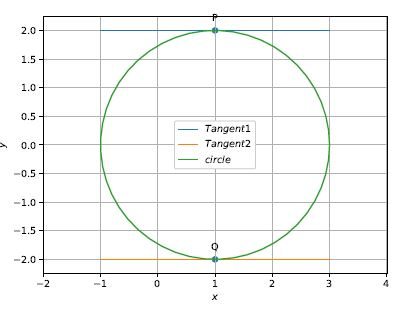
\includegraphics[width=\columnwidth]{./solutions/1/6/fig1.JPG}
	\caption{Figure depicting tangents of circle parallel to x-axis}
	\label{eq:solutions/1/6/fig1}
\end{figure}
